
\appendix
\newpage

\onecolumn
\begin{center}
    \vspace*{0.5cm}
    \LARGE{\bf{Supplementary Material \\ \Large{Noise-free Optimization in Early Training Steps for Image Super-Resolution}}} \\
    \vspace*{0.1cm}
    \bf{\Large{MinKyu Lee, Jae-Pil Heo\footnotemark[1]}} \\
    \vspace*{0.1cm}
    \large{\normalfont{Sungkyunkwan University}} \\
    \large{\normalfont{\{bluelati98, jaepilheo\}@skku.edu}}
    \vspace*{1.0cm}
\end{center}

\footnotetext{$^\ast$Corresponding author}



\begin{figure*}[h]
    \begin{center}
    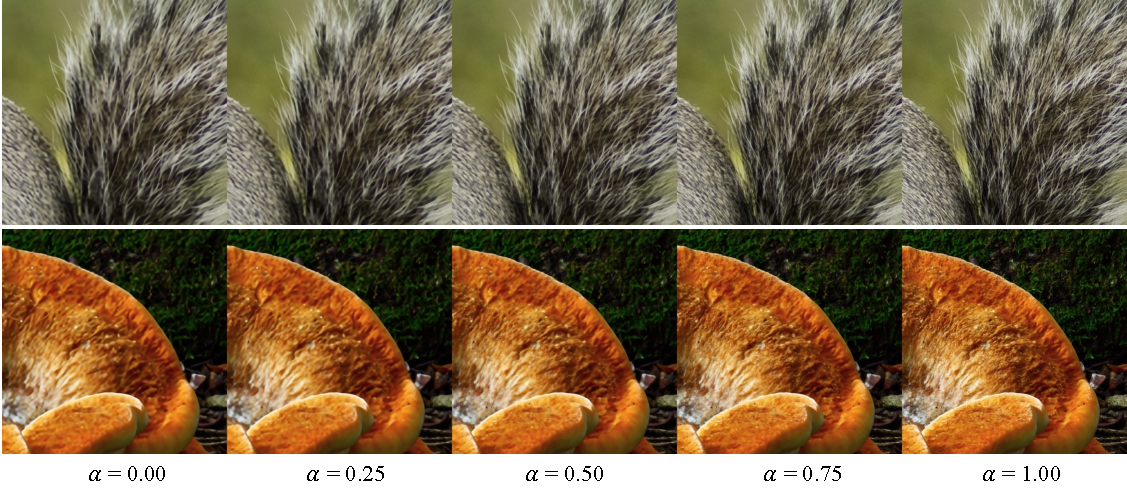
\includegraphics[width=\textwidth]{figures/alpha_visualize.pdf}
    \end{center}
    \vspace{-5pt}
    \caption{Visualization of target images in Eq.\eqref{eq:final_w_mixup} as $\alpha$ gradually changes. Unpredictable high-frequency components that can lead to unstable optimization are removed when $\alpha=0$. \textbf{Zoom in for best view.}}
    \label{fig:alpha_visualize}
\end{figure*}


\section{Visual Examples of Target Images\hfill\phantom{PLACEHOLDER}}

In order to perform noise-free training, the proposed training framework utilizes different target images as training proceeds. Specifically, the HR image and the SR image of a pretrained network are blended based on a scheduling parameter $\alpha$. In Fig.\ref{fig:alpha_visualize}, we provide visual examples of the target images in Eq.\eqref{eq:final_w_mixup} as $\alpha$ gradually changes from 0 to 1. As $\alpha$ increases, images become sharper but contain unpredictable high-frequency components, which can potentially lead to noisy and unstable training.




\section{Regressing the Inherent Noise\hfill\phantom{PLACEHOLDER}}
To determine the inherent noise $\epsilon^*$ of an HR image, a naive approach might involve training a network to regress the error term. Here we compare this naive approach of regressing the error against the proposed method ECO. The key distinction lies in the way each method approximates the noise.
Notably, the consequence of the regression is approximating the \textit{expectation} of the error $\mathbb{E}(\epsilon^*)$, given an \textbf{LR}. 
In contrast, ECO estimates $\epsilon^*$ directly, by utilizing \textbf{HR} at training time.
In Fig.\ref{fig:noise_comparison}, we visualize estimated $\mathbb{E}(\epsilon^*)$ and $\epsilon^*$. Here, $\mathbb{E}(\epsilon^*)$ is obtained by training an RRDB that is trained to regress $\epsilon^*$ instead of the SR image. It can be observed that $\mathbb{E}(\epsilon^*)$ results in a flat uncertainty map over the entire uncertain region. In contrast, $\epsilon^*$ better spots fine-grained noise factors, including almost invisible noise factors in the flat background. Note that we have shown how this noise can harm the training, underscoring the critical need for precise per-instance estimation of $\epsilon^*$.
%
\textbf{In a practical view}, estimating $\mathbb{E}(\epsilon^*)$ leads to significantly increased computational cost during training since it requires an additional network, whereas ECO only requires negligible cost. Specifically, the pretrained network $\hat{f}$ can be any off-the-shelf SR network for practical use cases, and $\mu_{emp}$ can be preprocessed before the actual training. 


\begin{figure}[h]
    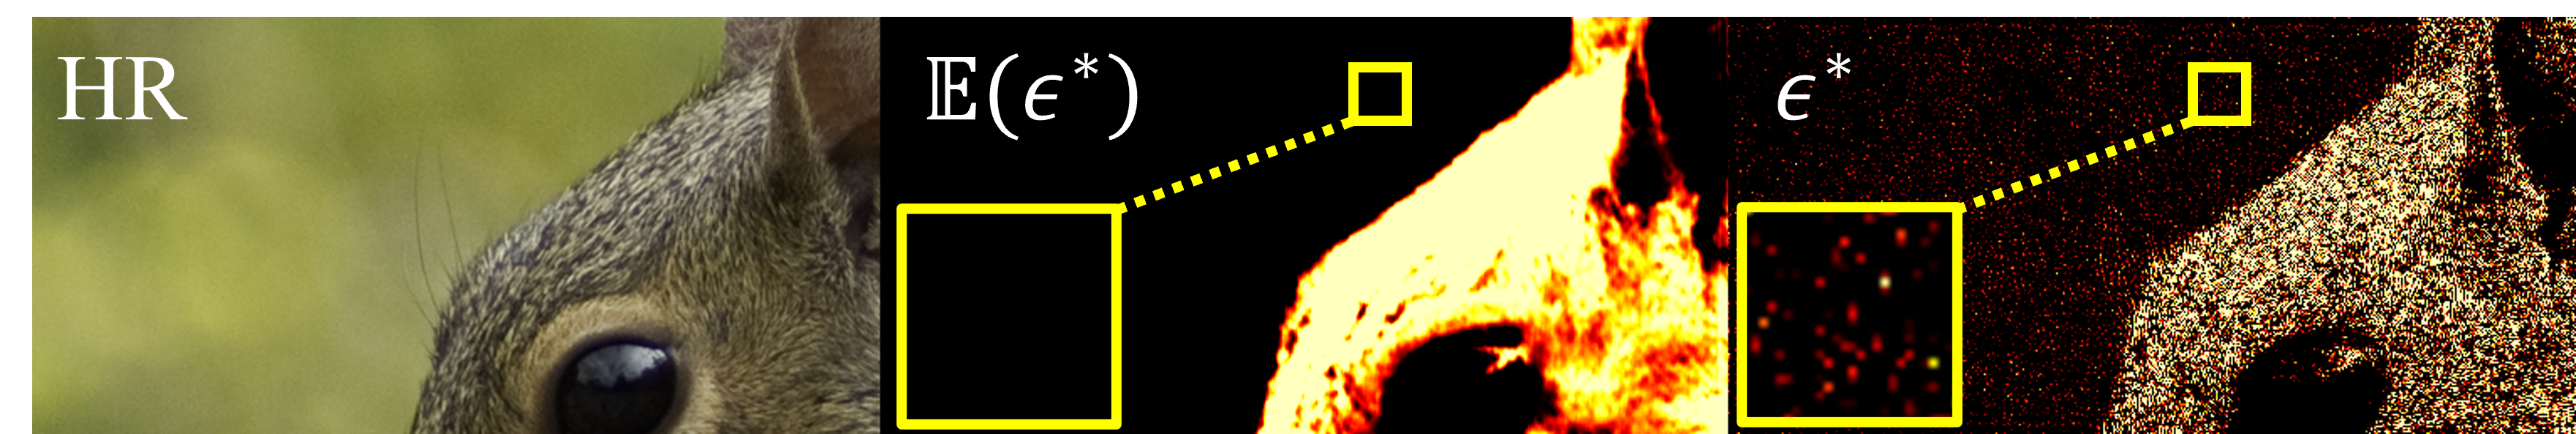
\includegraphics[width=\columnwidth]{figures/epsilon_vs_regression.png}
    \caption{
    Visualization of estimated $\mathbb{E}(\epsilon^*$) and $\epsilon^*$. It can be seen that $\epsilon^*$, which corresponds to the proposed method ECO, can better spot fine-grained noise factors including almost invisible noise in the flat background region. Values are scaled for better visualization. \textbf{Zoom in for best view}.
    }
    \label{fig:noise_comparison}
\end{figure}



\section{Analysis in the Spectral Domain\hfill\phantom{PLACEHOLDER}} \label{par:gradient_in_spectral_domain}

We provide further analysis to identify the specific components of image instances that affect the optimization procedure. To achieve this, we applied Fast Fourier Transform (FFT) directly followed by inverse FFT (IFFT) to the images before feeding them into the super-resolution network.
%
Fig.\ref{fig:high_frequency_gradient}.(a-b) illustrates HR, LR image pairs in the spectral domain and the gradients of losses in the spectral domain, both at $\alpha=0$.
%
Here, high activation on specific frequency regions indicates that the corresponding components are responsible for the loss values.
%
%
In the case of vanilla training, the gradients exhibit strong activation, particularly on the regions where \textit{very} high-frequency components exist. On the other hand, in ECO, while it is well activated on the major frequency components required for recovery, it shows relatively lower activation on very high-frequency components.
%
We interpret this as indicating the presence of inherent noise terms in the frequency domain.
%
%
By this observation, we conclude that ECO, indeed, has a powerful impact on the gradients, especially in regions where inherent noise terms are expected to reside.




\begin{figure*}[h]
    \begin{center}
    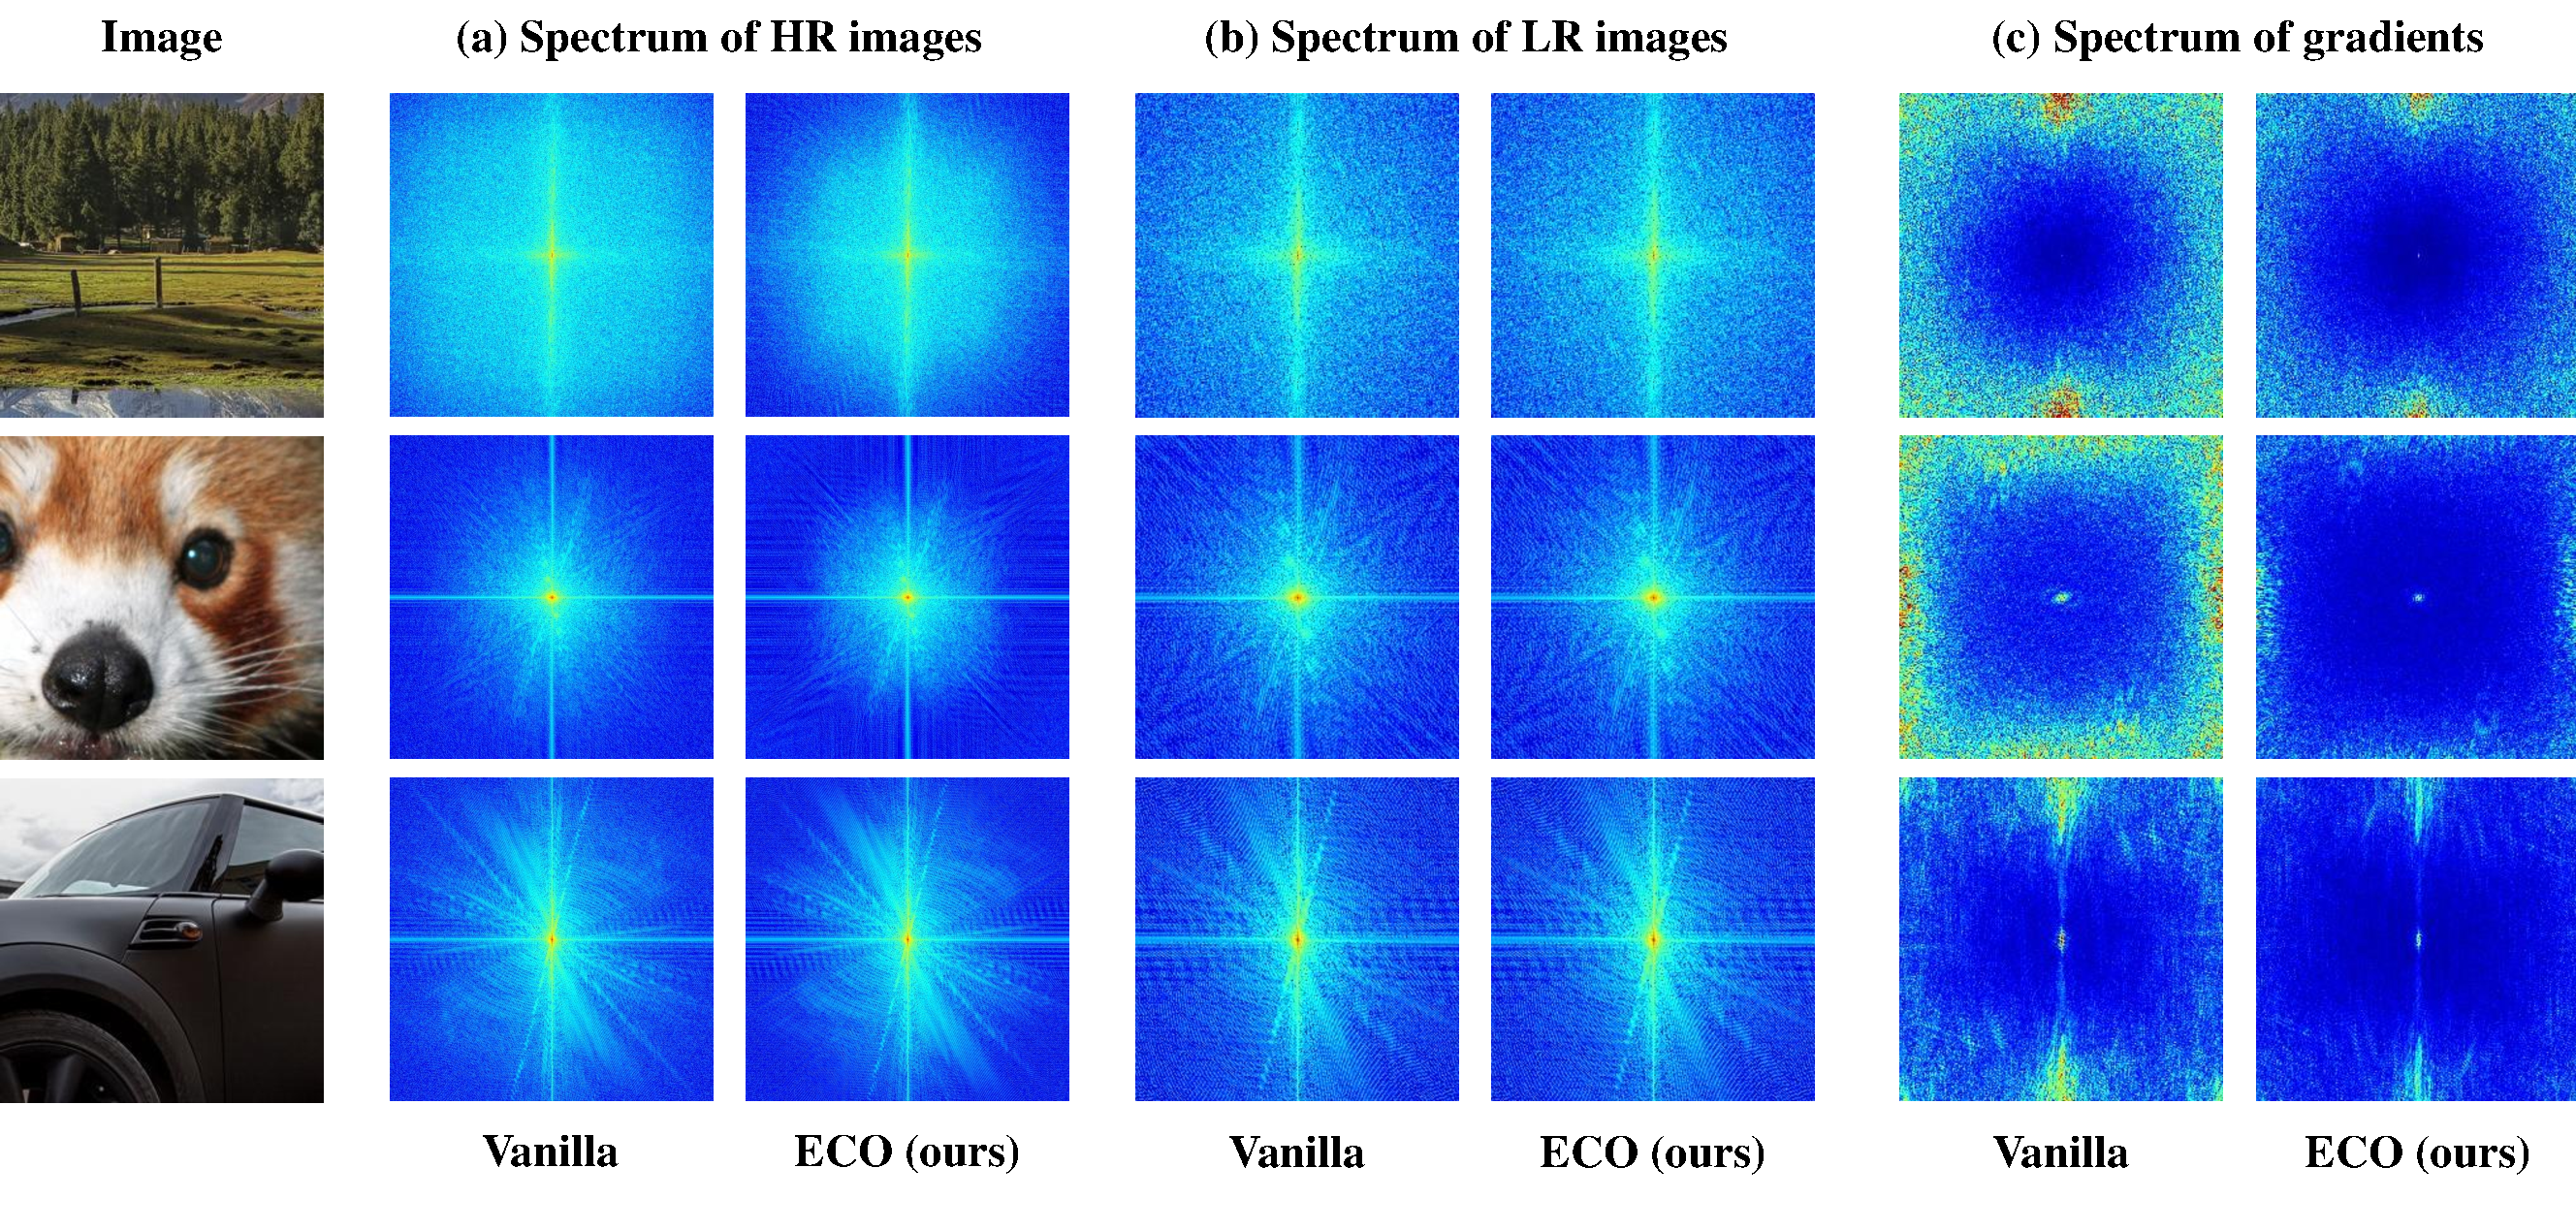
\includegraphics[width=\textwidth]{figures/high_frequency_gradient.pdf}
    \end{center}
    \vspace{-10pt}
    \caption{Spectral analysis of training data pairs and gradients at $\alpha=0$. (a) High-resolution images in the spectral domain. (b) Low-resolution images in the spectral domain. (c) The gradient of the loss in the spectral domain.}
    \label{fig:high_frequency_gradient}
\end{figure*}






\section{Experimental Details\hfill\phantom{PLACEHOLDER}}

\paragraph{Dataset details.}
For all datasets,  we generate LR images with the bicubic function in \text{MATLAB} with the antialiasing option set as true. We have verified that all LR and HR images match the images provided in the prior work \cite{SISR2_EDSR}. In the case of real-world SR, we add zero-mean color Gaussian noise with $\sigma=0.01$ to synthesize real-world images on flight. HR images were cropped modulo the scale factor in order to ensure that HR images match the output size of SR images.


\paragraph{Evaluation details.}
We have compared the proposed training scheme against vanilla training over standard benchmark datasets: Set5 \cite{set5}, Set14 \cite{set14}, BSD100 \cite{bsd100}, Urban100 \cite{urban100} and Manga109 \cite{manga109}. EDSR \cite{SISR2_EDSR}, RCAN \cite{SISR4_RCAN} and SwinIR \cite{liang2021swinir} were used as the representative baseline methods. Performances were evaluated in terms of PSNR and SSIM indices on the Y channel (luminance channel) in the YCbCr space and pixels up to the scale factors in the border were ignored. In the case of real-world SR, we provide average results of 10 different evaluation runs, where the test images were preprocessed for fair comparison.



\paragraph{Implementation details.}
For all experiments, we reproduce representative baseline networks EDSR-baseline, EDSR, RCAN and SwinIR with both vanilla training and our method. 
To train the networks, we use 800 RGB images from DIV2K \cite{div2k} and images were preprocessed as sub-patches for faster I/O. Note that we have only used the DIV2K dataset (instead of the DF2K) also for SwinIR, and do not use exponential moving averaged weights for both the baseline method and our method.
%
The patch size of low-resolution images was kept as 48$\times$48 for all scale factors as in prior works. Random horizontal and vertical flips were used, together with 90$^\circ$, 180$^\circ$, 270$^\circ$ random rotations as basic training augmentation. 
%
%
% ------------ training details
In Table.(1), we follow \cite{rcanit} which demonstrated comparable performance while significantly reducing the required training time.  We increase the learning rate by $\times$16 and the mini-batch size by $\times$8, decreasing the total training iteration by $\times$8. Specifically, the mini-batch size is 128, the learning rate is 0.0016, and the total training iteration is 125K.
%
We also substitute the scheduler as cosine annealing \cite{cosineannealing} and utilize the Lamb \cite{lamb} optimizer which is known to work better on larger batch sizes. We train our networks on two NVIDIA TITAN RTX GPUs and the batch size was selected to fit GPU memory. We train networks from scratch for $\times$2 SR. For $\times$3 SR and $\times$4 SR, we start from the pretrained weight of the $\times$2 SR network. 
%
However, for $\times$4 RCAN (both vanilla training and ours), we kept the setting of the original works \cite{SISR4_RCAN} since the baseline models produced undefined numbers (NaN) with larger learning rates. Specifically, the mini-batch size is 16, the learning rate is $10^{-4}$, the total training iteration is 1000K and the Adam optimizer was used and the learning rate was reduced by half every 200K iterations.
%
%
All networks in Tab.(1) were trained with two NVIDIA A6000 and all other networks were trained with one NVIDIA TITAN RTX.


